\documentclass[10pt,usepdftitle=false,aspectratio=169]{beamer}

% Preamble
%!TEX root = talk.tex

% Fonts and encoding
\usepackage[utf8]{inputenc} % allow utf-8 input
\usepackage[T1]{fontenc}    % use 8-bit T1 fonts
\usepackage{microtype}      % microtypography
\usepackage{inconsolata}
\usepackage[sfdefault,light,condensed]{roboto}
\usefonttheme[onlymath]{serif} % serif fonts for mathematics

% Enumerations and Items
\usepackage{enumitem}
\setitemize{label=\usebeamerfont*{itemize item}%
  \usebeamercolor[fg]{itemize item}
  \usebeamertemplate{itemize item}}
\usepackage{fourier-orns} % starred bullets

% Mathematics
\usepackage{amsmath}
\usepackage{amssymb}
\usepackage{amsfonts}       % blackboard math symbols
\usepackage{nicefrac}       % compact symbols for 1/2, etc.
\usepackage{mathtools}
\usepackage{relsize}
\usepackage{bm}
\usepackage{physics}
% Use "%%%%% MATH COMMANDS AND NOTATION %%%%%

\usepackage{amsmath}
\usepackage{amsfonts}
\usepackage{amssymb}
\usepackage{bm}
\usepackage{physics}

% Number Fields
\newcommand{\N}{\mathbb{N}}
\newcommand{\C}{\mathbb{C}}
\newcommand{\R}{\mathbb{R}}
\newcommand{\Q}{\mathbb{Q}}

% Common Linear Spaces
\newcommand{\Rn}{\mathbb{R}^n}
\newcommand{\Rd}{\mathbb{R}^d}
\newcommand{\Rnn}{\mathbb{R}^{n\times n}}
\newcommand{\Cn}{\mathbb{C}^n}
\newcommand{\Cnn}{\mathbb{C}^{n\times n}}

% Common Operators
\DeclareMathOperator{\sign}{sign}
\renewcommand{\top}{{\intercal}}
\def\ceil#1{\lceil #1 \rceil}
\def\floor#1{\lfloor #1 \rfloor}

% Vectorization and Kronecker-type products
\renewcommand{\vec}{\operatorname{vec}}
\newcommand{\svec}{\operatorname{svec}}
\newcommand{\smat}{\operatorname{smat}}
\newcommand{\mat}{\operatorname{mat}}
% to avoid warnings, copy only two symbols from stmaryrd
\DeclareSymbolFont{stmry}{U}{stmry}{m}{n}
\DeclareMathSymbol\obar\mathrel{stmry}{"3A}
\DeclareMathSymbol\otimes\mathrel{stmry}{"0F}
\DeclareMathSymbol\ominus\mathrel{stmry}{"17}
\makeatletter
\newcommand{\superimpose}[2]{%s
  {\ooalign{$#1\@firstoftwo#2$\cr\hfil$#1\@secondoftwo#2$\hfil\cr}}}
\makeatother
\newcommand{\ostimes}{\mathbin{\mathpalette\superimpose{{\otimes}{\ominus}}}}
\newcommand{\oatimes}{\mathbin{\mathpalette\superimpose{{\otimes}{\obar}}}}
\makeatother

% Probability
\renewcommand{\Pr}{\mathbb{P}}
\DeclareMathOperator{\Exp}{\mathbb{E}}
\DeclareMathOperator{\Var}{\mathrm{Var}}
\DeclareMathOperator{\Cov}{\mathrm{Cov}}
\DeclareMathOperator{\stderror}{\mathrm{SE}}
\DeclareMathOperator{\KL}{D_{\mathrm{KL}}}

\newcommand{\indep}{\perp\!\!\!\perp}

\newcommand{\Normal}{\mathcal{N}}
\newcommand{\GP}{\mathcal{GP}}
\newcommand{\subg}{\mathrm{subG}}
\newcommand{\Radem}{\mathrm{Radem}}
\newcommand{\Unif}{U}

% Optimization
\DeclareMathOperator*{\argmax}{arg\,max}
\DeclareMathOperator*{\argmin}{arg\,min}
\newcommand{\reg}{\lambda}

% Complexity and Asymptotics
\newcommand{\bigO}{\mathcal{O}}
\newcommand\smallO{
  \mathchoice
    {{\scriptstyle\mathcal{O}}}% \displaystyle
    {{\scriptstyle\mathcal{O}}}% \textstyle
    {{\scriptscriptstyle\mathcal{O}}}% \scriptstyle
    {\scalebox{.7}{$\scriptscriptstyle\mathcal{O}$}}%\scriptscriptstyle
  }
\newcommand{\bigTheta}{\Theta}
\newcommand{\bigOmega}{\Omega}
\newcommand{\smallOmega}{\omega}

% Random variables
\def\ra{{\mathsf{a}}}
\def\rb{{\mathsf{b}}}
\def\rc{{\mathsf{c}}}
\def\rd{{\mathsf{d}}}
\def\re{{\mathsf{e}}}
\def\rf{{\mathsf{f}}}
\def\rg{{\mathsf{g}}}
\def\rh{{\mathsf{h}}}
\def\ri{{\mathsf{i}}}
\def\rj{{\mathsf{j}}}
\def\rk{{\mathsf{k}}}
\def\rl{{\mathsf{l}}}
% rm is already a command, just don't name any random variables m
\def\rn{{\mathsf{n}}}
\def\ro{{\mathsf{o}}}
\def\rp{{\mathsf{p}}}
\def\rq{{\mathsf{q}}}
\def\rr{{\mathsf{r}}}
\def\rs{{\mathsf{s}}}
\def\rt{{\mathsf{t}}}
\def\ru{{\mathsf{u}}}
\def\rv{{\mathsf{v}}}
\def\rw{{\mathsf{w}}}
\def\rx{{\mathsf{x}}}
\def\ry{{\mathsf{y}}}
\def\rz{{\mathsf{z}}}

\def\reta{{\mathsf{$\eta$}}}

% Random vectors
\def\rva{{\bm{\mathsf{a}}}}
\def\rvb{{\bm{\mathsf{b}}}}
\def\rvc{{\bm{\mathsf{c}}}}
\def\rvd{{\bm{\mathsf{d}}}}
\def\rve{{\bm{\mathsf{e}}}}
\def\rvf{{\bm{\mathsf{f}}}}
\def\rvg{{\bm{\mathsf{g}}}}
\def\rvh{{\bm{\mathsf{h}}}}
\def\rvu{{\bm{\mathsf{i}}}}
\def\rvj{{\bm{\mathsf{j}}}}
\def\rvk{{\bm{\mathsf{k}}}}
\def\rvl{{\bm{\mathsf{l}}}}
\def\rvm{{\bm{\mathsf{m}}}}
\def\rvn{{\bm{\mathsf{n}}}}
\def\rvo{{\bm{\mathsf{o}}}}
\def\rvp{{\bm{\mathsf{p}}}}
\def\rvq{{\bm{\mathsf{q}}}}
\def\rvr{{\bm{\mathsf{r}}}}
\def\rvs{{\bm{\mathsf{s}}}}
\def\rvt{{\bm{\mathsf{t}}}}
\def\rvu{{\bm{\mathsf{u}}}}
\def\rvv{{\bm{\mathsf{v}}}}
\def\rvw{{\bm{\mathsf{w}}}}
\def\rvx{{\bm{\mathsf{x}}}}
\def\rvy{{\bm{\mathsf{y}}}}
\def\rvz{{\bm{\mathsf{z}}}}

\def\rvepsilon{{\bm{\mathsf{\epsilon}}}}
\def\rvtheta{{\bm{\mathsf{\theta}}}}

% Elements of random vectors
\def\erva{\bm{\mathsf{a}}}
\def\ervb{\bm{\mathsf{b}}}
\def\ervc{\bm{\mathsf{c}}}
\def\ervd{{\mathsf{d}}}
\def\erve{{\mathsf{e}}}
\def\ervf{{\mathsf{f}}}
\def\ervg{{\mathsf{g}}}
\def\ervh{{\mathsf{h}}}
\def\ervi{{\mathsf{i}}}
\def\ervj{{\mathsf{j}}}
\def\ervk{{\mathsf{k}}}
\def\ervl{{\mathsf{l}}}
\def\ervm{{\mathsf{m}}}
\def\ervn{{\mathsf{n}}}
\def\ervo{{\mathsf{o}}}
\def\ervp{{\mathsf{p}}}
\def\ervq{{\mathsf{q}}}
\def\ervr{{\mathsf{r}}}
\def\ervs{{\mathsf{s}}}
\def\ervt{{\mathsf{t}}}
\def\ervu{{\mathsf{u}}}
\def\ervv{{\mathsf{v}}}
\def\ervw{{\mathsf{w}}}
\def\ervx{{\mathsf{x}}}
\def\ervy{{\mathsf{y}}}
\def\ervz{{\mathsf{z}}}

% Random matrices
\def\rmA{{\bm{\mathsf{A}}}}
\def\rmB{{\bm{\mathsf{B}}}}
\def\rmC{{\bm{\mathsf{C}}}}
\def\rmD{{\bm{\mathsf{D}}}}
\def\rmE{{\bm{\mathsf{E}}}}
\def\rmF{{\bm{\mathsf{F}}}}
\def\rmG{{\bm{\mathsf{G}}}}
\def\rmH{{\bm{\mathsf{H}}}}
\def\rmI{{\bm{\mathsf{I}}}}
\def\rmJ{{\bm{\mathsf{J}}}}
\def\rmK{{\bm{\mathsf{K}}}}
\def\rmL{{\bm{\mathsf{L}}}}
\def\rmM{{\bm{\mathsf{M}}}}
\def\rmN{{\bm{\mathsf{N}}}}
\def\rmO{{\bm{\mathsf{O}}}}
\def\rmP{{\bm{\mathsf{P}}}}
\def\rmQ{{\bm{\mathsf{Q}}}}
\def\rmR{{\bm{\mathsf{R}}}}
\def\rmS{{\bm{\mathsf{S}}}}
\def\rmT{{\bm{\mathsf{T}}}}
\def\rmU{{\bm{\mathsf{U}}}}
\def\rmV{{\bm{\mathsf{V}}}}
\def\rmW{{\bm{\mathsf{W}}}}
\def\rmX{{\bm{\mathsf{X}}}}
\def\rmY{{\bm{\mathsf{Y}}}}
\def\rmZ{{\bm{\mathsf{Z}}}}

\def\rmBeta{{\bm{\mathsf{\beta}}}}
\def\rmPi{{\bm{\mathsf{\Pi}}}}
\def\rmPhi{{\bm{\mathsf{\Phi}}}}
\def\rmPsi{{\bm{\mathsf{\Psi}}}}
\def\rmLambda{{\bm{\mathsf{\Lambda}}}}
\def\rmSigma{{\bm{\mathsf{\Sigma}}}}
\def\rmDelta{{\bm{\mathsf{\Delta}}}}

% Elements of random matrices
\def\ermA{{\mathsf{A}}}
\def\ermB{{\mathsf{B}}}
\def\ermC{{\mathsf{C}}}
\def\ermD{{\mathsf{D}}}
\def\ermE{{\mathsf{E}}}
\def\ermF{{\mathsf{F}}}
\def\ermG{{\mathsf{G}}}
\def\ermH{{\mathsf{H}}}
\def\ermI{{\mathsf{I}}}
\def\ermJ{{\mathsf{J}}}
\def\ermK{{\mathsf{K}}}
\def\ermL{{\mathsf{L}}}
\def\ermM{{\mathsf{M}}}
\def\ermN{{\mathsf{N}}}
\def\ermO{{\mathsf{O}}}
\def\ermP{{\mathsf{P}}}
\def\ermQ{{\mathsf{Q}}}
\def\ermR{{\mathsf{R}}}
\def\ermS{{\mathsf{S}}}
\def\ermT{{\mathsf{T}}}
\def\ermU{{\mathsf{U}}}
\def\ermV{{\mathsf{V}}}
\def\ermW{{\mathsf{W}}}
\def\ermX{{\mathsf{X}}}
\def\ermY{{\mathsf{Y}}}
\def\ermZ{{\mathsf{Z}}}

% Vectors
\def\va{{\bm{a}}}
\def\vb{{\bm{b}}}
\def\vc{{\bm{c}}}
\def\vd{{\bm{d}}}
\def\ve{{\bm{e}}}
\def\vf{{\bm{\mathrm{f}}}}
\def\vg{{\bm{g}}}
\def\vh{{\bm{h}}}
\def\vi{{\bm{i}}}
\def\vj{{\bm{j}}}
\def\vk{{\bm{k}}}
\def\vl{{\bm{l}}}
\def\vm{{\bm{m}}}
\def\vn{{\bm{n}}}
\def\vo{{\bm{o}}}
\def\vp{{\bm{p}}}
\def\vq{{\bm{q}}}
\def\vr{{\bm{r}}}
\def\vs{{\bm{s}}}
\def\vt{{\bm{t}}}
\def\vu{{\bm{u}}}
\def\vv{{\bm{v}}}
\def\vw{{\bm{w}}}
\def\vx{{\bm{x}}}
\def\vy{{\bm{y}}}
\def\vz{{\bm{z}}}

\def\vmu{{\bm{\mu}}}
\def\vtheta{{\bm{\theta}}}
\def\valpha{{\bm{\alpha}}}
\def\vbeta{{\bm{\beta}}}
\def\vvarepsilon{{\bm{\varepsilon}}}
\def\vepsilon{{\bm{\epsilon}}}
\def\vgamma{{\bm{\gamma}}}
\def\vlambda{{\bm{\lambda}}}
\def\vphi{{\bm{\phi}}}
\def\vpsi{{\bm{\psi}}}
\def\vxi{{\bm{\xi}}}

\def\vzero{{\bm{0}}}
\def\vone{{\bm{1}}}

% Elements of vectors
\def\eva{{a}}
\def\evb{{b}}
\def\evc{{c}}
\def\evd{{d}}
\def\eve{{e}}
\def\evf{{f}}
\def\evg{{g}}
\def\evh{{h}}
\def\evi{{i}}
\def\evj{{j}}
\def\evk{{k}}
\def\evl{{l}}
\def\evm{{m}}
\def\evn{{n}}
\def\evo{{o}}
\def\evp{{p}}
\def\evq{{q}}
\def\evr{{r}}
\def\evs{{s}}
\def\evt{{t}}
\def\evu{{u}}
\def\evv{{v}}
\def\evw{{w}}
\def\evx{{x}}
\def\evy{{y}}
\def\evz{{z}}

\def\evalpha{{\alpha}}
\def\evbeta{{\beta}}
\def\evepsilon{{\epsilon}}
\def\evlambda{{\lambda}}
\def\evomega{{\omega}}
\def\evmu{{\mu}}
\def\evpsi{{\psi}}
\def\evsigma{{\sigma}}
\def\evtheta{{\theta}}
\def\evphi{{\phi}}
\def\evxi{{\xi}}

% Matrix
\def\mA{{\bm{A}}}
\def\mB{{\bm{B}}}
\def\mC{{\bm{C}}}
\def\mD{{\bm{D}}}
\def\mE{{\bm{E}}}
\def\mF{{\bm{F}}}
\def\mG{{\bm{G}}}
\def\mH{{\bm{H}}}
\def\mI{{\bm{I}}}
\def\mJ{{\bm{J}}}
\def\mK{{\bm{K}}}
\def\mL{{\bm{L}}}
\def\mM{{\bm{M}}}
\def\mN{{\bm{N}}}
\def\mO{{\bm{O}}}
\def\mP{{\bm{P}}}
\def\mQ{{\bm{Q}}}
\def\mR{{\bm{R}}}
\def\mS{{\bm{S}}}
\def\mT{{\bm{T}}}
\def\mU{{\bm{U}}}
\def\mV{{\bm{V}}}
\def\mW{{\bm{W}}}
\def\mX{{\bm{X}}}
\def\mY{{\bm{Y}}}
\def\mZ{{\bm{Z}}}

\def\mBeta{{\bm{\beta}}}
\def\mGamma{{\bm{\Gamma}}}
\def\mDelta{{\bm{\Delta}}}
\def\mEpsilon{{\bm{\mathcal{E}}}}
\def\mPi{{\bm{\Pi}}}
\def\mPhi{{\bm{\Phi}}}
\def\mPsi{{\bm{\Psi}}}
\def\mLambda{{\bm{\Lambda}}}
\def\mSigma{{\bm{\Sigma}}}

% Tensor
\DeclareMathAlphabet{\mathsfit}{\encodingdefault}{\sfdefault}{m}{sl}
\SetMathAlphabet{\mathsfit}{bold}{\encodingdefault}{\sfdefault}{bx}{n}
\newcommand{\tens}[1]{\bm{\mathsfit{#1}}}
\def\tA{{\tens{A}}}
\def\tB{{\tens{B}}}
\def\tC{{\tens{C}}}
\def\tD{{\tens{D}}}
\def\tE{{\tens{E}}}
\def\tF{{\tens{F}}}
\def\tG{{\tens{G}}}
\def\tH{{\tens{H}}}
\def\tI{{\tens{I}}}
\def\tJ{{\tens{J}}}
\def\tK{{\tens{K}}}
\def\tL{{\tens{L}}}
\def\tM{{\tens{M}}}
\def\tN{{\tens{N}}}
\def\tO{{\tens{O}}}
\def\tP{{\tens{P}}}
\def\tQ{{\tens{Q}}}
\def\tR{{\tens{R}}}
\def\tS{{\tens{S}}}
\def\tT{{\tens{T}}}
\def\tU{{\tens{U}}}
\def\tV{{\tens{V}}}
\def\tW{{\tens{W}}}
\def\tX{{\tens{X}}}
\def\tY{{\tens{Y}}}
\def\tZ{{\tens{Z}}}


% Graph
\def\gA{{\mathcal{A}}}
\def\gB{{\mathcal{B}}}
\def\gC{{\mathcal{C}}}
\def\gD{{\mathcal{D}}}
\def\gE{{\mathcal{E}}}
\def\gF{{\mathcal{F}}}
\def\gG{{\mathcal{G}}}
\def\gH{{\mathcal{H}}}
\def\gI{{\mathcal{I}}}
\def\gJ{{\mathcal{J}}}
\def\gK{{\mathcal{K}}}
\def\gL{{\mathcal{L}}}
\def\gM{{\mathcal{M}}}
\def\gN{{\mathcal{N}}}
\def\gO{{\mathcal{O}}}
\def\gP{{\mathcal{P}}}
\def\gQ{{\mathcal{Q}}}
\def\gR{{\mathcal{R}}}
\def\gS{{\mathcal{S}}}
\def\gT{{\mathcal{T}}}
\def\gU{{\mathcal{U}}}
\def\gV{{\mathcal{V}}}
\def\gW{{\mathcal{W}}}
\def\gX{{\mathcal{X}}}
\def\gY{{\mathcal{Y}}}
\def\gZ{{\mathcal{Z}}}

% Sets
\def\sA{{A}}
\def\sB{{B}}
\def\sC{{C}}
\def\sD{{D}}
% Don't use a set called E, because this would be the same as our symbol
% for expectation.
\def\sF{{F}}
\def\sG{{G}}
\def\sH{{H}}
\def\sI{{I}}
\def\sJ{{J}}
\def\sK{{K}}
\def\sL{{L}}
\def\sM{{M}}
\def\sN{{N}}
\def\sO{{O}}
\def\sP{{P}}
\def\sQ{{Q}}
\def\sR{{R}}
\def\sS{{S}}
\def\sT{{T}}
\def\sU{{U}}
\def\sV{{V}}
\def\sW{{W}}
\def\sX{{X}}
\def\sY{{Y}}
\def\sZ{{Z}}

% Entries of a matrix
\def\emA{{A}}
\def\emB{{B}}
\def\emC{{C}}
\def\emD{{D}}
\def\emE{{E}}
\def\emF{{F}}
\def\emG{{G}}
\def\emH{{H}}
\def\emI{{I}}
\def\emJ{{J}}
\def\emK{{K}}
\def\emL{{L}}
\def\emM{{M}}
\def\emN{{N}}
\def\emO{{O}}
\def\emP{{P}}
\def\emQ{{Q}}
\def\emR{{R}}
\def\emS{{S}}
\def\emT{{T}}
\def\emU{{U}}
\def\emV{{V}}
\def\emW{{W}}
\def\emX{{X}}
\def\emY{{Y}}
\def\emZ{{Z}}

\def\emSigma{{\Sigma}}
\def\emLambda{{\Lambda}}

% entries of a tensor
% Same font as tensor, without \bm wrapper
\newcommand{\etens}[1]{\mathsfit{#1}}
\def\etA{{\etens{A}}}
\def\etB{{\etens{B}}}
\def\etC{{\etens{C}}}
\def\etD{{\etens{D}}}
\def\etE{{\etens{E}}}
\def\etF{{\etens{F}}}
\def\etG{{\etens{G}}}
\def\etH{{\etens{H}}}
\def\etI{{\etens{I}}}
\def\etJ{{\etens{J}}}
\def\etK{{\etens{K}}}
\def\etL{{\etens{L}}}
\def\etM{{\etens{M}}}
\def\etN{{\etens{N}}}
\def\etO{{\etens{O}}}
\def\etP{{\etens{P}}}
\def\etQ{{\etens{Q}}}
\def\etR{{\etens{R}}}
\def\etS{{\etens{S}}}
\def\etT{{\etens{T}}}
\def\etU{{\etens{U}}}
\def\etV{{\etens{V}}}
\def\etW{{\etens{W}}}
\def\etX{{\etens{X}}}
\def\etY{{\etens{Y}}}
\def\etZ{{\etens{Z}}}

\def\etLambda{{\etens{\Lambda}}}


\let\ab\allowbreak
" in the main tex file to include further notational commands.

% Figures
\usepackage{graphicx}
\usepackage{pgfplots}
\pgfplotsset{compat=1.15}
\usepackage{caption}
\captionsetup[table]{skip=5pt}
\usepackage{subcaption}

% Tikz
\usepackage{etoolbox}
\robustify\bfseries
\usepackage{pgfplots}
\usepgfplotslibrary{groupplots,patchplots}
\usepackage{tikz}
\usetikzlibrary{tikzmark}
\usetikzlibrary{calc}

% % Tikz externalize
% \usetikzlibrary{external}
% \tikzexternalize[mode=list and make]
% % use  "make -j 8 -f main.makefile" to compile with 8 parallel threads (this is what it takes to max out the machine, despite it having 4 cores)
% \tikzset{external/force remake=false}
% \tikzsetexternalprefix{figures/external/}

% Plot dimensions
\newlength{\figureheight}
\newlength{\figurewidth}
\newlength{\figheight}
\newlength{\figwidth}

% Tables
\usepackage{booktabs}
\usepackage{rotating}
\usepackage{siunitx}
\sisetup{
  tight-spacing=true,
  output-exponent-marker=\text{e},
  exponent-product={},
  group-separator = {,},
  mode=text,
}
%\renewcommand{\arraystretch}{1.5} % Increase table row height
\usepackage{multirow}

% Algorithms
\usepackage{algorithm}% http://ctan.org/pkg/algorithm
\usepackage{algpseudocode}% http://ctan.org/pkg/algorithmicx
\algrenewcommand{\algorithmiccomment}[1]{\hfill {\textcolor{darkgray}{\scriptsize \# #1}}}
%\algrenewcommand\alglinenumber[1]{\tiny #1}

% Symbols
\newcommand{\cmark}{}%
\DeclareRobustCommand{\cmark}{%
  \tikz\fill[scale=0.4, color=black!30!green]
  (0,.35) -- (.25,0) -- (1,.7) -- (.25,.15) -- cycle;%
}
\newcommand{\xmark}{}%
\DeclareRobustCommand{\xmark}{%
  \tikz [x=1.4ex,y=1.4ex,line width=.2ex, color=red] \draw (0,0) -- (1,1) (0,1) -- (1,0);
}
\newcommand{\umark}{{\color{orange}\(\thicksim\)}}

% References and Bibliography
\usepackage{url}
\usepackage{xr}
\usepackage{hyperref}
% \hypersetup{
%   colorlinks,
%   linkcolor={black},
%   citecolor={blue!50!black},
%   urlcolor={blue!50!black}
% }
\usepackage{cleveref}
\usepackage{bookmark} % Fixes false PDF table of contents
\usepackage{natbib}
\setcitestyle{authoryear,square,comma,numbers,sort&compress}
\renewcommand*{\bibfont}{\small} % fontsize references
\usepackage{bibentry}
\nobibliography*

% Colors
\usepackage{xcolor, colortbl}
\definecolor{lred}{RGB}{200,0,0}
\definecolor{dred}{RGB}{130,0,0}
\definecolor{dblu}{RGB}{0,0,130}
\definecolor{dgre}{RGB}{0,130,0}
\definecolor{dgra}{RGB}{50,50,50}
\definecolor{mgra}{RGB}{221,222,214}
\definecolor{lgra}{RGB}{238,238,234}
\definecolor{MPG}{RGB}{000,125,122}
\definecolor{lMPG}{RGB}{000,190,189}
\definecolor{ora}{HTML}{FF9933} %EI orange
\definecolor{lblu}{HTML}{7DA7D9}%PS blue
% Color scheme of the Eberhard-Karls University
\definecolor{TUred}{RGB}{141,45,57}
\definecolor{TUdark}{RGB}{55,65,74}
\definecolor{TUgold}{RGB}{174,159,109}
\definecolor{TUgray}{RGB}{175,179,183}
\definecolor{ERC_ora}{RGB}{233,93,15}
\setlength{\parindent}{0pt}

\newcommand{\mpg}[1]{{\color{MPG} #1}}   % highlight command 1
\newcommand{\dre}[1]{{\color{TUred} #1}}   % highlight command 1
\newcommand{\blu}[1]{{\color{dblu} #1}}   % highlight command 1
\newcommand{\ora}[1]{{\color{ora} #1}}   % highlight command 1
\newcommand{\gra}[1]{{\color{mgra} #1}}   % highlight command 1
\newcommand{\gold}[1]{{\color{TUgold} #1}}   % highlight command 1
\setbeamercolor{alerted text}{fg = TUred} % highlight command 2
\setbeamercolor{normal text}{fg=black,bg=white}
\setbeamercolor{structure}{fg=TUred}
\setbeamercolor{item projected}{use=item,fg=black,bg = TUred}
\setbeamercolor*{palette primary}{fg=white,bg=TUred}
\setbeamercolor*{palette secondary}{parent=palette primary,use=palette
  primary,bg=dblu}
\setbeamercolor*{palette tertiary}{parent=palette
  primary,use=palette primary,fg=white,bg=dgre}
\setbeamercolor*{palette
  quaternary}{parent=palette primary,use=palette primary,bg=dgre}
\setbeamercolor*{block body}{bg=TUgray, fg =black}
\setbeamercolor*{block title}{parent=structure,bg=TUdark,fg=white}
\setbeamercolor{block body alerted}{bg=TUgray,fg=TUred}
\setbeamercolor{block title example}{fg=MPG,bg=white}
\setbeamercolor{block body example}{fg=black,bg=white}
\setbeamercolor{frametitle}{bg=TUdark,fg=white}
\setbeamercolor{frametitle right}{bg=white}
\setbeamercolor{framesubtitle}{fg=TUgray}
\setbeamercolor{title}{fg=TUred}
\setbeamercolor{subtitle}{fg=black} \setbeamercolor{author}{fg=TUdark}
\setbeamercolor{date}{fg=TUdark}
\setbeamercolor*{titlelike}{parent=structure}

%------------ Beamer template settings and commands ------------%

% Text
\let\emph\relax % redefine \emph to COLORS. % there's no \RedeclareTextFontCommand
\DeclareTextFontCommand{\emph}{\color{TUred}}

% Enumerations
\setbeamertemplate{itemize items}{\starredbullet}

% Table of Contents
\setbeamertemplate{section in toc}{\vspace{.75em} \inserttocsection \par}

% Bibliography
\setbeamertemplate{bibliography item}[triangle]

% General
\setbeamertemplate{navigation symbols}{}
\setbeamerfont{frametitle}{}
\setbeamertemplate{footline}{\hfill\color{TUdark}{\insertframenumber}\hspace{2ex}\null\newline\vspace{2mm}}
\arrayrulecolor{TUdark}

\newcommand{\filltotal}{\hspace{0pt plus 1 filll}}
\newcommand{\titlemark}[1]{
  \begin{tikzpicture}[remember picture, overlay]
    \node[draw=none,text=TUgray,anchor=north east,yshift=-.8259cm] at (current
    page.north east) {\footnotesize{#1}};
  \end{tikzpicture}
}
\newcommand{\graybox}[1]{
  \tikzexternaldisable%
  \begin{center}%
    \tikz{\node[fill=TUdark,text width=\textwidth]{%
        \begin{minipage}{1.0\linewidth}%
          \color{white}
          \begin{center}%
            #1
          \end{center}%
        \end{minipage}};}%
  \end{center}%
  \tikzexternalenable
}
\newcommand{\divider}{\noindent\makebox[\linewidth]{\rule{\paperwidth}{.4pt}}  }
\newcommand{\paperwhite}{\includegraphics[height=.6\baselineskip]{../text-document_white.png}\hspace{.5em}}
\newcommand{\paperblack}{\includegraphics[height=.6\baselineskip]{../text-document.png}\hspace{.5em}}
\newcommand{\bookwhite}{\includegraphics[height=.6\baselineskip]{../book-white.png}\hspace{.5em}}
\newcommand{\bookblack}{\includegraphics[height=.6\baselineskip]{../book-black.png}\hspace{.5em}}

\setbeamercolor{ribboncolor}{fg=black,bg=TUgold}
\newcommand{\ribbon}[1]{
  \begin{beamercolorbox}[wd=\paperwidth,colsep*=.3em,center]{ribboncolor}
    \setbeamertemplate{itemize items}{\color{black}\starredbullet}
    \setbeamercolor{structure}{fg=white}
    \begin{minipage}{1.0\textwidth}%
      #1
    \end{minipage}
  \end{beamercolorbox}
}
\setbeamercolor{whiteribboncolor}{fg=black,bg=white}
\newcommand{\whiteribbon}[1]{
  \begin{beamercolorbox}[wd=\paperwidth,colsep*=.5em,center]{whiteribboncolor}
    \setbeamertemplate{itemize items}{\color{black}\starredbullet}
    \setbeamercolor{structure}{fg=black}
    \begin{minipage}{\textwidth}%
      #1
    \end{minipage}
  \end{beamercolorbox}
}
\newcommand{\bfa}[1]{
  \begin{beamercolorbox}[wd=\paperwidth,colsep*=.5em,center]{white}
    \setbeamertemplate{itemize items}{\color{black}\starredbullet}
    \tikzexternaldisable
    \begin{tikzpicture}
      \node[signal,minimum width=\paperwidth,draw=TUgold,fill=TUgold,text=black,text width=\textwidth]{
        \begin{minipage}{\textwidth}%
          #1
        \end{minipage}};
    \end{tikzpicture}
    \tikzexternalenable
  \end{beamercolorbox}
}
\newcommand{\bfi}[1]{
  \begin{beamercolorbox}[wd=\paperwidth,colsep*=.5em,center]{white}
    \setbeamertemplate{itemize items}{\color{black}\starredbullet}
    \tikzexternaldisable
    \begin{tikzpicture}
      \node[signal,signal from=west,signal to=nowhere,minimum width=\linewidth,draw=TUgold,fill=TUgold,text=black,signal pointer angle=140]{
        \begin{minipage}{\textwidth}%
          #1
        \end{minipage}};
    \end{tikzpicture}\hspace{2.5mm}
    \tikzexternalenable
  \end{beamercolorbox}
}
\newcommand{\blackslide}{
  {\setbeamercolor{background canvas}{bg=black}
      \begin{frame}[plain]
        \null
      \end{frame}
    }}
\newcommand{\blackslidetext}[1]{
  {\setbeamercolor{background canvas}{bg=TUdark}%
      \setbeamercolor{structure}{fg=white}%
      \setbeamercolor{normal text}{fg=white}%
      \setbeamercolor{body}{fg=white}%
      \setbeamercolor{itemize/enumerate body}{fg=white}%
      \setbeamertemplate{itemize items}{\color{white}\starredbullet}%
      \begin{frame}
        \color{white} #1
      \end{frame}
    }}
% logo in the upper right corner
\usepackage{eso-pic}
\newcommand\AtPagemyUpperLeft[1]{\AtPageLowerLeft{%
    \put(\LenToUnit{0.83\paperwidth},\LenToUnit{0.915\paperheight}){#1}}}
\AddToShipoutPictureFG{
  \AtPagemyUpperLeft{{
\includegraphics[width=2.5cm,keepaspectratio]{assets/UT_WBMW_Weiss_1C.pdf}}}
}%
%%%%% MATH COMMANDS AND NOTATION %%%%%

\usepackage{amsmath}
\usepackage{amsfonts}
\usepackage{amssymb}
\usepackage{bm}
\usepackage{physics}

% Number Fields
\newcommand{\N}{\mathbb{N}}
\newcommand{\C}{\mathbb{C}}
\newcommand{\R}{\mathbb{R}}
\newcommand{\Q}{\mathbb{Q}}

% Common Linear Spaces
\newcommand{\Rn}{\mathbb{R}^n}
\newcommand{\Rd}{\mathbb{R}^d}
\newcommand{\Rnn}{\mathbb{R}^{n\times n}}
\newcommand{\Cn}{\mathbb{C}^n}
\newcommand{\Cnn}{\mathbb{C}^{n\times n}}

% Common Operators
\DeclareMathOperator{\sign}{sign}
\renewcommand{\top}{{\intercal}}
\def\ceil#1{\lceil #1 \rceil}
\def\floor#1{\lfloor #1 \rfloor}

% Vectorization and Kronecker-type products
\renewcommand{\vec}{\operatorname{vec}}
\newcommand{\svec}{\operatorname{svec}}
\newcommand{\smat}{\operatorname{smat}}
\newcommand{\mat}{\operatorname{mat}}
% to avoid warnings, copy only two symbols from stmaryrd
\DeclareSymbolFont{stmry}{U}{stmry}{m}{n}
\DeclareMathSymbol\obar\mathrel{stmry}{"3A}
\DeclareMathSymbol\otimes\mathrel{stmry}{"0F}
\DeclareMathSymbol\ominus\mathrel{stmry}{"17}
\makeatletter
\newcommand{\superimpose}[2]{%s
  {\ooalign{$#1\@firstoftwo#2$\cr\hfil$#1\@secondoftwo#2$\hfil\cr}}}
\makeatother
\newcommand{\ostimes}{\mathbin{\mathpalette\superimpose{{\otimes}{\ominus}}}}
\newcommand{\oatimes}{\mathbin{\mathpalette\superimpose{{\otimes}{\obar}}}}
\makeatother

% Probability
\renewcommand{\Pr}{\mathbb{P}}
\DeclareMathOperator{\Exp}{\mathbb{E}}
\DeclareMathOperator{\Var}{\mathrm{Var}}
\DeclareMathOperator{\Cov}{\mathrm{Cov}}
\DeclareMathOperator{\stderror}{\mathrm{SE}}
\DeclareMathOperator{\KL}{D_{\mathrm{KL}}}

\newcommand{\indep}{\perp\!\!\!\perp}

\newcommand{\Normal}{\mathcal{N}}
\newcommand{\GP}{\mathcal{GP}}
\newcommand{\subg}{\mathrm{subG}}
\newcommand{\Radem}{\mathrm{Radem}}
\newcommand{\Unif}{U}

% Optimization
\DeclareMathOperator*{\argmax}{arg\,max}
\DeclareMathOperator*{\argmin}{arg\,min}
\newcommand{\reg}{\lambda}

% Complexity and Asymptotics
\newcommand{\bigO}{\mathcal{O}}
\newcommand\smallO{
  \mathchoice
    {{\scriptstyle\mathcal{O}}}% \displaystyle
    {{\scriptstyle\mathcal{O}}}% \textstyle
    {{\scriptscriptstyle\mathcal{O}}}% \scriptstyle
    {\scalebox{.7}{$\scriptscriptstyle\mathcal{O}$}}%\scriptscriptstyle
  }
\newcommand{\bigTheta}{\Theta}
\newcommand{\bigOmega}{\Omega}
\newcommand{\smallOmega}{\omega}

% Random variables
\def\ra{{\mathsf{a}}}
\def\rb{{\mathsf{b}}}
\def\rc{{\mathsf{c}}}
\def\rd{{\mathsf{d}}}
\def\re{{\mathsf{e}}}
\def\rf{{\mathsf{f}}}
\def\rg{{\mathsf{g}}}
\def\rh{{\mathsf{h}}}
\def\ri{{\mathsf{i}}}
\def\rj{{\mathsf{j}}}
\def\rk{{\mathsf{k}}}
\def\rl{{\mathsf{l}}}
% rm is already a command, just don't name any random variables m
\def\rn{{\mathsf{n}}}
\def\ro{{\mathsf{o}}}
\def\rp{{\mathsf{p}}}
\def\rq{{\mathsf{q}}}
\def\rr{{\mathsf{r}}}
\def\rs{{\mathsf{s}}}
\def\rt{{\mathsf{t}}}
\def\ru{{\mathsf{u}}}
\def\rv{{\mathsf{v}}}
\def\rw{{\mathsf{w}}}
\def\rx{{\mathsf{x}}}
\def\ry{{\mathsf{y}}}
\def\rz{{\mathsf{z}}}

\def\reta{{\mathsf{$\eta$}}}

% Random vectors
\def\rva{{\bm{\mathsf{a}}}}
\def\rvb{{\bm{\mathsf{b}}}}
\def\rvc{{\bm{\mathsf{c}}}}
\def\rvd{{\bm{\mathsf{d}}}}
\def\rve{{\bm{\mathsf{e}}}}
\def\rvf{{\bm{\mathsf{f}}}}
\def\rvg{{\bm{\mathsf{g}}}}
\def\rvh{{\bm{\mathsf{h}}}}
\def\rvu{{\bm{\mathsf{i}}}}
\def\rvj{{\bm{\mathsf{j}}}}
\def\rvk{{\bm{\mathsf{k}}}}
\def\rvl{{\bm{\mathsf{l}}}}
\def\rvm{{\bm{\mathsf{m}}}}
\def\rvn{{\bm{\mathsf{n}}}}
\def\rvo{{\bm{\mathsf{o}}}}
\def\rvp{{\bm{\mathsf{p}}}}
\def\rvq{{\bm{\mathsf{q}}}}
\def\rvr{{\bm{\mathsf{r}}}}
\def\rvs{{\bm{\mathsf{s}}}}
\def\rvt{{\bm{\mathsf{t}}}}
\def\rvu{{\bm{\mathsf{u}}}}
\def\rvv{{\bm{\mathsf{v}}}}
\def\rvw{{\bm{\mathsf{w}}}}
\def\rvx{{\bm{\mathsf{x}}}}
\def\rvy{{\bm{\mathsf{y}}}}
\def\rvz{{\bm{\mathsf{z}}}}

\def\rvepsilon{{\bm{\mathsf{\epsilon}}}}
\def\rvtheta{{\bm{\mathsf{\theta}}}}

% Elements of random vectors
\def\erva{\bm{\mathsf{a}}}
\def\ervb{\bm{\mathsf{b}}}
\def\ervc{\bm{\mathsf{c}}}
\def\ervd{{\mathsf{d}}}
\def\erve{{\mathsf{e}}}
\def\ervf{{\mathsf{f}}}
\def\ervg{{\mathsf{g}}}
\def\ervh{{\mathsf{h}}}
\def\ervi{{\mathsf{i}}}
\def\ervj{{\mathsf{j}}}
\def\ervk{{\mathsf{k}}}
\def\ervl{{\mathsf{l}}}
\def\ervm{{\mathsf{m}}}
\def\ervn{{\mathsf{n}}}
\def\ervo{{\mathsf{o}}}
\def\ervp{{\mathsf{p}}}
\def\ervq{{\mathsf{q}}}
\def\ervr{{\mathsf{r}}}
\def\ervs{{\mathsf{s}}}
\def\ervt{{\mathsf{t}}}
\def\ervu{{\mathsf{u}}}
\def\ervv{{\mathsf{v}}}
\def\ervw{{\mathsf{w}}}
\def\ervx{{\mathsf{x}}}
\def\ervy{{\mathsf{y}}}
\def\ervz{{\mathsf{z}}}

% Random matrices
\def\rmA{{\bm{\mathsf{A}}}}
\def\rmB{{\bm{\mathsf{B}}}}
\def\rmC{{\bm{\mathsf{C}}}}
\def\rmD{{\bm{\mathsf{D}}}}
\def\rmE{{\bm{\mathsf{E}}}}
\def\rmF{{\bm{\mathsf{F}}}}
\def\rmG{{\bm{\mathsf{G}}}}
\def\rmH{{\bm{\mathsf{H}}}}
\def\rmI{{\bm{\mathsf{I}}}}
\def\rmJ{{\bm{\mathsf{J}}}}
\def\rmK{{\bm{\mathsf{K}}}}
\def\rmL{{\bm{\mathsf{L}}}}
\def\rmM{{\bm{\mathsf{M}}}}
\def\rmN{{\bm{\mathsf{N}}}}
\def\rmO{{\bm{\mathsf{O}}}}
\def\rmP{{\bm{\mathsf{P}}}}
\def\rmQ{{\bm{\mathsf{Q}}}}
\def\rmR{{\bm{\mathsf{R}}}}
\def\rmS{{\bm{\mathsf{S}}}}
\def\rmT{{\bm{\mathsf{T}}}}
\def\rmU{{\bm{\mathsf{U}}}}
\def\rmV{{\bm{\mathsf{V}}}}
\def\rmW{{\bm{\mathsf{W}}}}
\def\rmX{{\bm{\mathsf{X}}}}
\def\rmY{{\bm{\mathsf{Y}}}}
\def\rmZ{{\bm{\mathsf{Z}}}}

\def\rmBeta{{\bm{\mathsf{\beta}}}}
\def\rmPi{{\bm{\mathsf{\Pi}}}}
\def\rmPhi{{\bm{\mathsf{\Phi}}}}
\def\rmPsi{{\bm{\mathsf{\Psi}}}}
\def\rmLambda{{\bm{\mathsf{\Lambda}}}}
\def\rmSigma{{\bm{\mathsf{\Sigma}}}}
\def\rmDelta{{\bm{\mathsf{\Delta}}}}

% Elements of random matrices
\def\ermA{{\mathsf{A}}}
\def\ermB{{\mathsf{B}}}
\def\ermC{{\mathsf{C}}}
\def\ermD{{\mathsf{D}}}
\def\ermE{{\mathsf{E}}}
\def\ermF{{\mathsf{F}}}
\def\ermG{{\mathsf{G}}}
\def\ermH{{\mathsf{H}}}
\def\ermI{{\mathsf{I}}}
\def\ermJ{{\mathsf{J}}}
\def\ermK{{\mathsf{K}}}
\def\ermL{{\mathsf{L}}}
\def\ermM{{\mathsf{M}}}
\def\ermN{{\mathsf{N}}}
\def\ermO{{\mathsf{O}}}
\def\ermP{{\mathsf{P}}}
\def\ermQ{{\mathsf{Q}}}
\def\ermR{{\mathsf{R}}}
\def\ermS{{\mathsf{S}}}
\def\ermT{{\mathsf{T}}}
\def\ermU{{\mathsf{U}}}
\def\ermV{{\mathsf{V}}}
\def\ermW{{\mathsf{W}}}
\def\ermX{{\mathsf{X}}}
\def\ermY{{\mathsf{Y}}}
\def\ermZ{{\mathsf{Z}}}

% Vectors
\def\va{{\bm{a}}}
\def\vb{{\bm{b}}}
\def\vc{{\bm{c}}}
\def\vd{{\bm{d}}}
\def\ve{{\bm{e}}}
\def\vf{{\bm{\mathrm{f}}}}
\def\vg{{\bm{g}}}
\def\vh{{\bm{h}}}
\def\vi{{\bm{i}}}
\def\vj{{\bm{j}}}
\def\vk{{\bm{k}}}
\def\vl{{\bm{l}}}
\def\vm{{\bm{m}}}
\def\vn{{\bm{n}}}
\def\vo{{\bm{o}}}
\def\vp{{\bm{p}}}
\def\vq{{\bm{q}}}
\def\vr{{\bm{r}}}
\def\vs{{\bm{s}}}
\def\vt{{\bm{t}}}
\def\vu{{\bm{u}}}
\def\vv{{\bm{v}}}
\def\vw{{\bm{w}}}
\def\vx{{\bm{x}}}
\def\vy{{\bm{y}}}
\def\vz{{\bm{z}}}

\def\vmu{{\bm{\mu}}}
\def\vtheta{{\bm{\theta}}}
\def\valpha{{\bm{\alpha}}}
\def\vbeta{{\bm{\beta}}}
\def\vvarepsilon{{\bm{\varepsilon}}}
\def\vepsilon{{\bm{\epsilon}}}
\def\vgamma{{\bm{\gamma}}}
\def\vlambda{{\bm{\lambda}}}
\def\vphi{{\bm{\phi}}}
\def\vpsi{{\bm{\psi}}}
\def\vxi{{\bm{\xi}}}

\def\vzero{{\bm{0}}}
\def\vone{{\bm{1}}}

% Elements of vectors
\def\eva{{a}}
\def\evb{{b}}
\def\evc{{c}}
\def\evd{{d}}
\def\eve{{e}}
\def\evf{{f}}
\def\evg{{g}}
\def\evh{{h}}
\def\evi{{i}}
\def\evj{{j}}
\def\evk{{k}}
\def\evl{{l}}
\def\evm{{m}}
\def\evn{{n}}
\def\evo{{o}}
\def\evp{{p}}
\def\evq{{q}}
\def\evr{{r}}
\def\evs{{s}}
\def\evt{{t}}
\def\evu{{u}}
\def\evv{{v}}
\def\evw{{w}}
\def\evx{{x}}
\def\evy{{y}}
\def\evz{{z}}

\def\evalpha{{\alpha}}
\def\evbeta{{\beta}}
\def\evepsilon{{\epsilon}}
\def\evlambda{{\lambda}}
\def\evomega{{\omega}}
\def\evmu{{\mu}}
\def\evpsi{{\psi}}
\def\evsigma{{\sigma}}
\def\evtheta{{\theta}}
\def\evphi{{\phi}}
\def\evxi{{\xi}}

% Matrix
\def\mA{{\bm{A}}}
\def\mB{{\bm{B}}}
\def\mC{{\bm{C}}}
\def\mD{{\bm{D}}}
\def\mE{{\bm{E}}}
\def\mF{{\bm{F}}}
\def\mG{{\bm{G}}}
\def\mH{{\bm{H}}}
\def\mI{{\bm{I}}}
\def\mJ{{\bm{J}}}
\def\mK{{\bm{K}}}
\def\mL{{\bm{L}}}
\def\mM{{\bm{M}}}
\def\mN{{\bm{N}}}
\def\mO{{\bm{O}}}
\def\mP{{\bm{P}}}
\def\mQ{{\bm{Q}}}
\def\mR{{\bm{R}}}
\def\mS{{\bm{S}}}
\def\mT{{\bm{T}}}
\def\mU{{\bm{U}}}
\def\mV{{\bm{V}}}
\def\mW{{\bm{W}}}
\def\mX{{\bm{X}}}
\def\mY{{\bm{Y}}}
\def\mZ{{\bm{Z}}}

\def\mBeta{{\bm{\beta}}}
\def\mGamma{{\bm{\Gamma}}}
\def\mDelta{{\bm{\Delta}}}
\def\mEpsilon{{\bm{\mathcal{E}}}}
\def\mPi{{\bm{\Pi}}}
\def\mPhi{{\bm{\Phi}}}
\def\mPsi{{\bm{\Psi}}}
\def\mLambda{{\bm{\Lambda}}}
\def\mSigma{{\bm{\Sigma}}}

% Tensor
\DeclareMathAlphabet{\mathsfit}{\encodingdefault}{\sfdefault}{m}{sl}
\SetMathAlphabet{\mathsfit}{bold}{\encodingdefault}{\sfdefault}{bx}{n}
\newcommand{\tens}[1]{\bm{\mathsfit{#1}}}
\def\tA{{\tens{A}}}
\def\tB{{\tens{B}}}
\def\tC{{\tens{C}}}
\def\tD{{\tens{D}}}
\def\tE{{\tens{E}}}
\def\tF{{\tens{F}}}
\def\tG{{\tens{G}}}
\def\tH{{\tens{H}}}
\def\tI{{\tens{I}}}
\def\tJ{{\tens{J}}}
\def\tK{{\tens{K}}}
\def\tL{{\tens{L}}}
\def\tM{{\tens{M}}}
\def\tN{{\tens{N}}}
\def\tO{{\tens{O}}}
\def\tP{{\tens{P}}}
\def\tQ{{\tens{Q}}}
\def\tR{{\tens{R}}}
\def\tS{{\tens{S}}}
\def\tT{{\tens{T}}}
\def\tU{{\tens{U}}}
\def\tV{{\tens{V}}}
\def\tW{{\tens{W}}}
\def\tX{{\tens{X}}}
\def\tY{{\tens{Y}}}
\def\tZ{{\tens{Z}}}


% Graph
\def\gA{{\mathcal{A}}}
\def\gB{{\mathcal{B}}}
\def\gC{{\mathcal{C}}}
\def\gD{{\mathcal{D}}}
\def\gE{{\mathcal{E}}}
\def\gF{{\mathcal{F}}}
\def\gG{{\mathcal{G}}}
\def\gH{{\mathcal{H}}}
\def\gI{{\mathcal{I}}}
\def\gJ{{\mathcal{J}}}
\def\gK{{\mathcal{K}}}
\def\gL{{\mathcal{L}}}
\def\gM{{\mathcal{M}}}
\def\gN{{\mathcal{N}}}
\def\gO{{\mathcal{O}}}
\def\gP{{\mathcal{P}}}
\def\gQ{{\mathcal{Q}}}
\def\gR{{\mathcal{R}}}
\def\gS{{\mathcal{S}}}
\def\gT{{\mathcal{T}}}
\def\gU{{\mathcal{U}}}
\def\gV{{\mathcal{V}}}
\def\gW{{\mathcal{W}}}
\def\gX{{\mathcal{X}}}
\def\gY{{\mathcal{Y}}}
\def\gZ{{\mathcal{Z}}}

% Sets
\def\sA{{A}}
\def\sB{{B}}
\def\sC{{C}}
\def\sD{{D}}
% Don't use a set called E, because this would be the same as our symbol
% for expectation.
\def\sF{{F}}
\def\sG{{G}}
\def\sH{{H}}
\def\sI{{I}}
\def\sJ{{J}}
\def\sK{{K}}
\def\sL{{L}}
\def\sM{{M}}
\def\sN{{N}}
\def\sO{{O}}
\def\sP{{P}}
\def\sQ{{Q}}
\def\sR{{R}}
\def\sS{{S}}
\def\sT{{T}}
\def\sU{{U}}
\def\sV{{V}}
\def\sW{{W}}
\def\sX{{X}}
\def\sY{{Y}}
\def\sZ{{Z}}

% Entries of a matrix
\def\emA{{A}}
\def\emB{{B}}
\def\emC{{C}}
\def\emD{{D}}
\def\emE{{E}}
\def\emF{{F}}
\def\emG{{G}}
\def\emH{{H}}
\def\emI{{I}}
\def\emJ{{J}}
\def\emK{{K}}
\def\emL{{L}}
\def\emM{{M}}
\def\emN{{N}}
\def\emO{{O}}
\def\emP{{P}}
\def\emQ{{Q}}
\def\emR{{R}}
\def\emS{{S}}
\def\emT{{T}}
\def\emU{{U}}
\def\emV{{V}}
\def\emW{{W}}
\def\emX{{X}}
\def\emY{{Y}}
\def\emZ{{Z}}

\def\emSigma{{\Sigma}}
\def\emLambda{{\Lambda}}

% entries of a tensor
% Same font as tensor, without \bm wrapper
\newcommand{\etens}[1]{\mathsfit{#1}}
\def\etA{{\etens{A}}}
\def\etB{{\etens{B}}}
\def\etC{{\etens{C}}}
\def\etD{{\etens{D}}}
\def\etE{{\etens{E}}}
\def\etF{{\etens{F}}}
\def\etG{{\etens{G}}}
\def\etH{{\etens{H}}}
\def\etI{{\etens{I}}}
\def\etJ{{\etens{J}}}
\def\etK{{\etens{K}}}
\def\etL{{\etens{L}}}
\def\etM{{\etens{M}}}
\def\etN{{\etens{N}}}
\def\etO{{\etens{O}}}
\def\etP{{\etens{P}}}
\def\etQ{{\etens{Q}}}
\def\etR{{\etens{R}}}
\def\etS{{\etens{S}}}
\def\etT{{\etens{T}}}
\def\etU{{\etens{U}}}
\def\etV{{\etens{V}}}
\def\etW{{\etens{W}}}
\def\etX{{\etens{X}}}
\def\etY{{\etens{Y}}}
\def\etZ{{\etens{Z}}}

\def\etLambda{{\etens{\Lambda}}}


\let\ab\allowbreak


% Code Highlighting
\usepackage{pythonhighlight}

% Information
\def\myemail{jonathan.wenger@uni-tuebingen.de}
\def\mywebsite{jonathanwenger.netlify.app}
\def\mygithub{JonathanWenger}


\begin{document}

% \tikzexternaldisable
\begin{frame}
	\vspace{.5cm}
	\title{
		{\bf Probabilistic Numerical Methods}\newline An Algorithmic Perspective
		\vspace*{-.7cm}}
	\author{\bf Jonathan Wenger\vspace{-1cm}} \date{MCM 2021\\ August 19, 2021}

	%\vspace{-1.5cm}
	\maketitle
	%\vspace{1.em}

	\begin{columns}
		\column{0.45\textwidth}
		
\includegraphics[width=\textwidth]{assets/UT_WBMW_Rot_RGB.pdf}
		\column{.45\textwidth}
		
\includegraphics[width=.9\textwidth]{assets/MPI-IS_wortbildmarke.png}\\
		\parbox[c]{.1\textwidth}{\centering
\includegraphics[height=1.05cm]{assets/imprs-is-logo.png}}
	\end{columns}

	\thispagestyle{empty}
	\setcounter{framenumber}{0}

	%%%%%%%%%%%%%%%% ANIMATED LOGO %%%%%%%%%%%%%%%%
	%  \tikzifexternalizing{}{%
	%  \begin{tikzpicture}[remember picture,overlay]
	%  \node[anchor=south,yshift=-5mm] at (current page.south) 
	%  {\animategraphics[width=0.9995\paperwidth,autoplay,loop]{36}{assets/logo_TU_169_}{0}{39}};
	%    \end{tikzpicture}%
	%  }%
	% if you don't like the animation or it doesn't work for you, use this here instead:
	\begin{columns}
		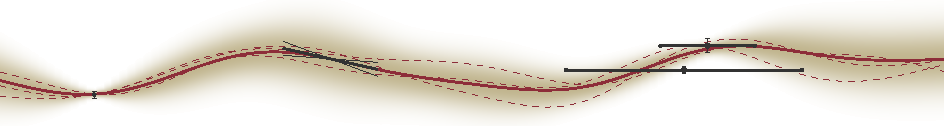
\includegraphics[width=0.9995\paperwidth]{assets/logo_TU_169_0.pdf}
	\end{columns}
	%%%%%%%%%%%%%% END OF ANIMATED LOGO %%%%%%%%%%%

\end{frame}
% \tikzexternalenable

\section{Probabilistic Numerical Methods}

\subsection{What and Why?}

\begin{frame}\frametitle{What is a Probabilistic Numerical Method?}
	\framesubtitle{\dots and why should I care?}

	\begin{block}{}
		\emph{\bf Numerical methods} that return \emph{\bf probability measures} designed to
		quantify numerical error.
	\end{block}

	\vspace{1em}

	\begin{columns}

		\column{0.66\textwidth}

		\emph{Advantages}
		\begin{itemize}
			\item \textit{structural uncertainty} via a probability measure compared to an error estimate
			\item \textit{customized methods} for specific problems with bespoke priors
			\item set \textit{parameters of numerical methods} via the Bayesian formalism
			\item solution of \textit{mutually related problems} of similar type
			\item incorporate \textit{sources of stochasticity} in the computation
		\end{itemize}

		\column{0.33\textwidth}

		\centering

		\adjustbox{max width=0.9\textwidth, valign=c}{
			\tikzset{every picture/.style={line width=0.75pt}} %set default line width to 0.75pt        

		\begin{tikzpicture}[
				x=0.75pt,
				y=0.75pt,
				yscale=-1,
				xscale=1,
			]
			%uncomment if require: \path (0,245); %set diagram left start at 0, and has height of 245

			%Shape: Parallelogram [id:dp0484593371293055] 
			\draw  [fill={rgb, 255:red, 0; green, 0; blue, 0 }	,fill opacity=0.2 ] (36.37,218.7) -- (36.37,128) -- (218.37,-1.09) -- (218.37,89.61) -- cycle ;
			%Straight Lines [id:da8755796520304125] 
			\draw [color={rgb, 255:red, 128; green, 128; blue, 128 }	,draw opacity=1 ][fill={rgb, 255:red, 0; green, 0; blue, 0 }	,fill opacity=0.2 ]   (75,16) -- (128.92,106.76) ;
			\draw [shift={(128.92,106.76)}, rotate = 59.29] [color={rgb, 255:red, 128; green, 128; blue, 128 }	,draw opacity=1 ][fill={rgb, 255:red, 128; green, 128; blue, 128 }	,fill opacity=1 ][line width=0.75]      (0, 0) circle [x radius= 3.35, y radius= 3.35]	;
			%Straight Lines [id:da17763309372062497] 
			\draw [color={rgb, 255:red, 128; green, 128; blue, 128 }	,draw opacity=1 ][fill={rgb, 255:red, 0; green, 0; blue, 0 }	,fill opacity=0.2 ]   (148,139) -- (187.37,206.85) ;

			%Shape: Ellipse [id:dp3096241264352757] 
			\draw  [color={rgb, 255:red, 74; green, 108; blue, 226 }	,draw opacity=0.5 ][fill={rgb, 255:red, 255; green, 255; blue, 255 }  ,fill opacity=0.2 ][line width=1.5]  (45.3,163.6) .. controls (39.06,154.41) and (71.43,121.51) .. (117.6,90.12) .. controls
			(163.78,58.73) and (206.28,40.73) .. (212.53,49.92) .. controls (218.78,59.11) and (186.41,92.01)
			.. (140.23,123.4) .. controls (94.05,154.8) and (51.55,172.8) .. (45.3,163.6) -- cycle ;
			%Straight Lines [id:da7512972710991653] 
			\draw  [dash pattern={on 4.5pt off 4.5pt}]  (75,16) -- (127.9,105.04) ;
			\draw [shift={(128.92,106.76)}, rotate = 239.29] [fill={rgb, 255:red, 0; green, 0; blue, 0 }  ][line width=0.08]  [draw opacity=0] (12,-3) -- (0,0) -- (12,3) -- cycle    ;
			\draw [shift={(75,16)}, rotate = 59.29] [color={rgb, 255:red, 0; green, 0; blue, 0 }  ][fill={rgb, 255:red, 0; green, 0; blue, 0 }  ][line width=0.75]      (0, 0) circle [x radius= 3.35, y radius= 3.35]	;
			%Straight Lines [id:da6115370118887071] 
			\draw  [dash pattern={on 4.5pt off 4.5pt}]  (63.37,151.85) -- (127.27,107.89) ;
			\draw [shift={(128.92,106.76)}, rotate = 505.48] [fill={rgb, 255:red, 0; green, 0; blue, 0 }  ][line width=0.08]  [draw opacity=0] (12,-3) -- (0,0) -- (12,3) -- cycle    ;
			\draw [shift={(63.37,151.85)}, rotate = 325.48] [color={rgb, 255:red, 0; green, 0; blue, 0 }  ][fill={rgb, 255:red, 0; green, 0; blue, 0 }  ][line width=0.75]      (0, 0) circle [x radius= 3.35, y radius= 3.35]	 ;
			%Shape: Ellipse [id:dp22358481605415048] 
			\draw  [color={rgb, 255:red, 74; green, 108; blue, 226 }  ,draw opacity=0.5 ][line width=1.5]  (99.97,126.44) .. controls (97.81,123.26) and (109.01,111.87) .. (125,101) .. controls
			(140.99,90.13) and (155.7,83.9) .. (157.86,87.08) .. controls (160.02,90.26) and (148.82,101.65) ..
			(132.83,112.52) .. controls (116.85,123.39) and (102.14,129.62) .. (99.97,126.44) -- cycle ;
			%Shape: Ellipse [id:dp6795155838154404] 
			\draw  [color={rgb, 255:red, 74; green, 108; blue, 226 }  ,draw opacity=0.5 ][line width=1.5]  (75.88,143.81) .. controls (72.03,138.15) and (91.96,117.89) .. (120.4,98.56) .. controls
			(148.84,79.23) and (175.01,68.14) .. (178.85,73.8) .. controls (182.7,79.46) and (162.77,99.72) ..
			(134.33,119.05) .. controls (105.9,138.38) and (79.73,149.47) .. (75.88,143.81) -- cycle ;

			% Text Node
			\draw (135,97) node [anchor=north west][inner sep=0.75pt]  [font=\Large]  {$\vx_{k+1}$};
			% Text Node
			\draw (50,157) node [anchor=north west][inner sep=0.75pt]  [font=\Large]  {$\vx_*$};
			% Text Node
			\draw (87,5.4) node [anchor=north west][inner sep=0.75pt]  [font=\Large]  {$\vx_k$};

		\end{tikzpicture}
		}

	\end{columns}

	\vspace{1.8em}

	\ribbon{\centering \textbf{Vision:} Propagation of uncertainty through chains of computations.}

\end{frame}

\subsection{Components of a PNM}

\begin{frame}\frametitle{Components of a (Bayesian) PN Method}
	\framesubtitle{}

	\begin{columns}[c,totalwidth=\textwidth]
		\column{.45\textwidth}

		\emph{Components}
		\begin{itemize}
			\item Prior Knowledge
			\item Policy
			\item Action and Observation
			\item Posterior Inference
			\item Stopping Criterion
			\item Hyperparameter Optimization

		\end{itemize}

		\column{.5\textwidth}
		\centering
		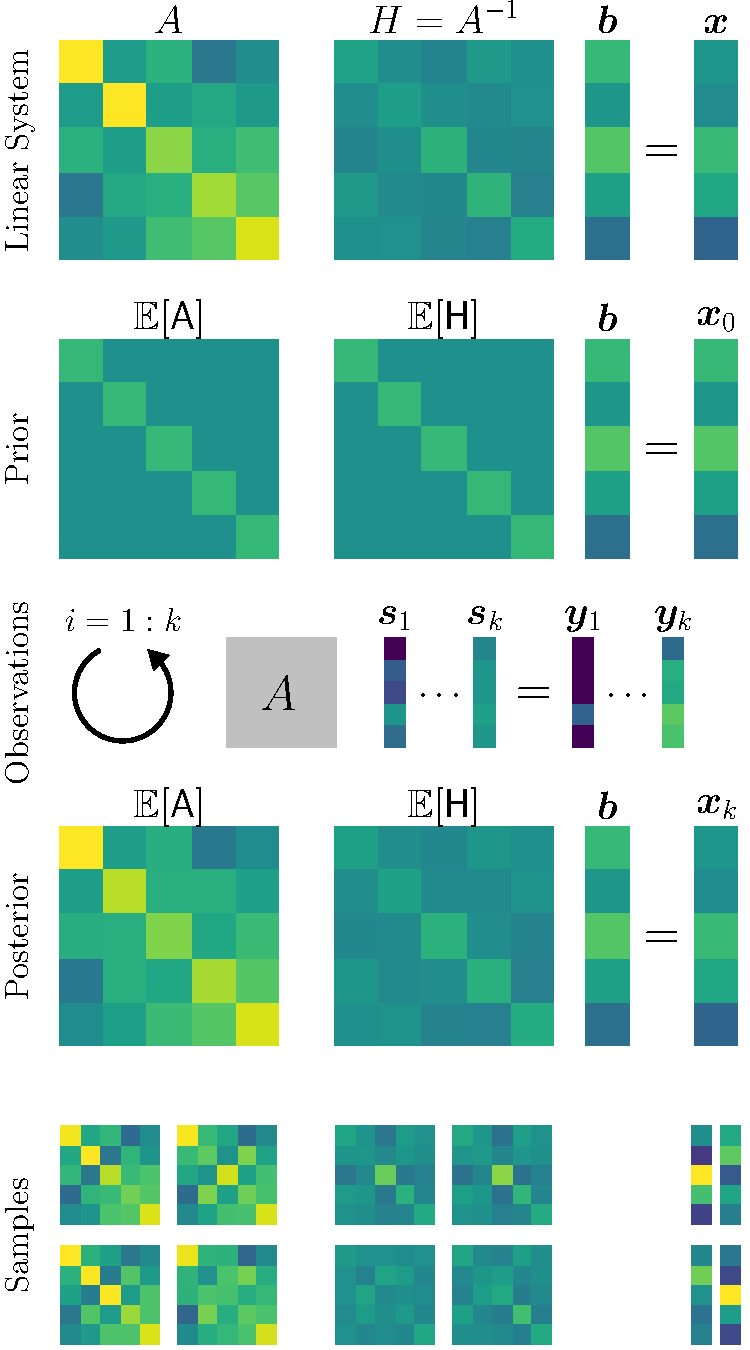
\includegraphics[width=0.6\textwidth]{figures/problinsolve.pdf}

	\end{columns}

\end{frame}

\subsection{Formal Definition}

\begin{frame}\frametitle{But what \textit{exactly} is a PN Method?}
	\framesubtitle{A formal definition and an algorithmic translation.}

	\begin{columns}[totalwidth=\textwidth]
		\column{.45\textwidth}

		\begin{definition}[\citet{Cockayne2019a}]
			Let \((\mathcal{X}, \Sigma_\mathcal{X})\),
			\((\mathcal{A}, \Sigma_\mathcal{A})\) and \((\mathcal{Q},
			\Sigma_\mathcal{Q})\) be measurable spaces and \(X\) a random variable on
			\((\mathcal{X}, \Sigma_\mathcal{X})\). Take
			\(\mu(B)=\mathbb{P}(\{w : X(w) \in B\})\) to be the law of \(X\). Further, let
			\(A:\mathcal{X} \rightarrow \mathcal{A}\), \(Q: \mathcal{X}
			\rightarrow \mathcal{Q}\) and \(B: \mathcal{P}_\mathcal{X} \times
			\mathcal{A} \rightarrow \mathcal{P}_\mathcal{Q}\) where \(A\) and
			\(Q\) are measurable functions.
			\vspace{1.5ex}

			The pair \(M=(A,B)\) is called a \emph{probabilistic numerical method} for estimation of a quantity of interest
			\(Q\). The map \(A\) is called an \emph{information operator}, and the map \(B\) is called a
			\emph{belief update operator}.
		\end{definition}

		\column{.05\textwidth}

		\column{.5\textwidth}

		\textbf{Goal:} Given a problem \(F(\vx) = 0\), return a quantity of interest \(q(\vx)\).

		\setcounter{algorithm}{0}
		\begin{algorithm}[H]
			\caption{Probabilistic Numerical Method}
			\small
			\begin{algorithmic}[1]
				\Procedure{\textsc{ProbNumMethod}}{$F(\cdot), \rvx$}
				\Comment{problem \& prior}
				\While{\textbf{not} \textsc{HasConverged}($F, \rvx, \rvq$)}	%\Comment{stopping criteria}
				\State \({\vs} \gets \textsc{Policy}(F, \rvx, \rvq)\)
				\Comment{action via policy}
				\State \({\vy} \gets\) \textsc{InformationOp}($F$, $\rvx$, $\rvq$, $\vs$)
				% \Comment{observation}
				\State {\color{gray} \(\theta_* \gets \) \textsc{HyperparamOptim}($\theta, \mS, \mY$)}
				\State \(\rvq \gets \textsc{BeliefUpdate}((\vs, \vy), \rvx, F,
				{\color{gray}\theta_*})\)
				% \Comment{posterior}
				\EndWhile
				\State \Return $\rvq$
				\EndProcedure
			\end{algorithmic}
		\end{algorithm}

	\end{columns}

\end{frame}

\section{Software for PN}

\subsection{ProbNum}

\begin{frame}\frametitle{ProbNum}
	\framesubtitle{Probabilistic Numerics in Python.}
	\vspace{-0.35em}
	\makebox[\linewidth]{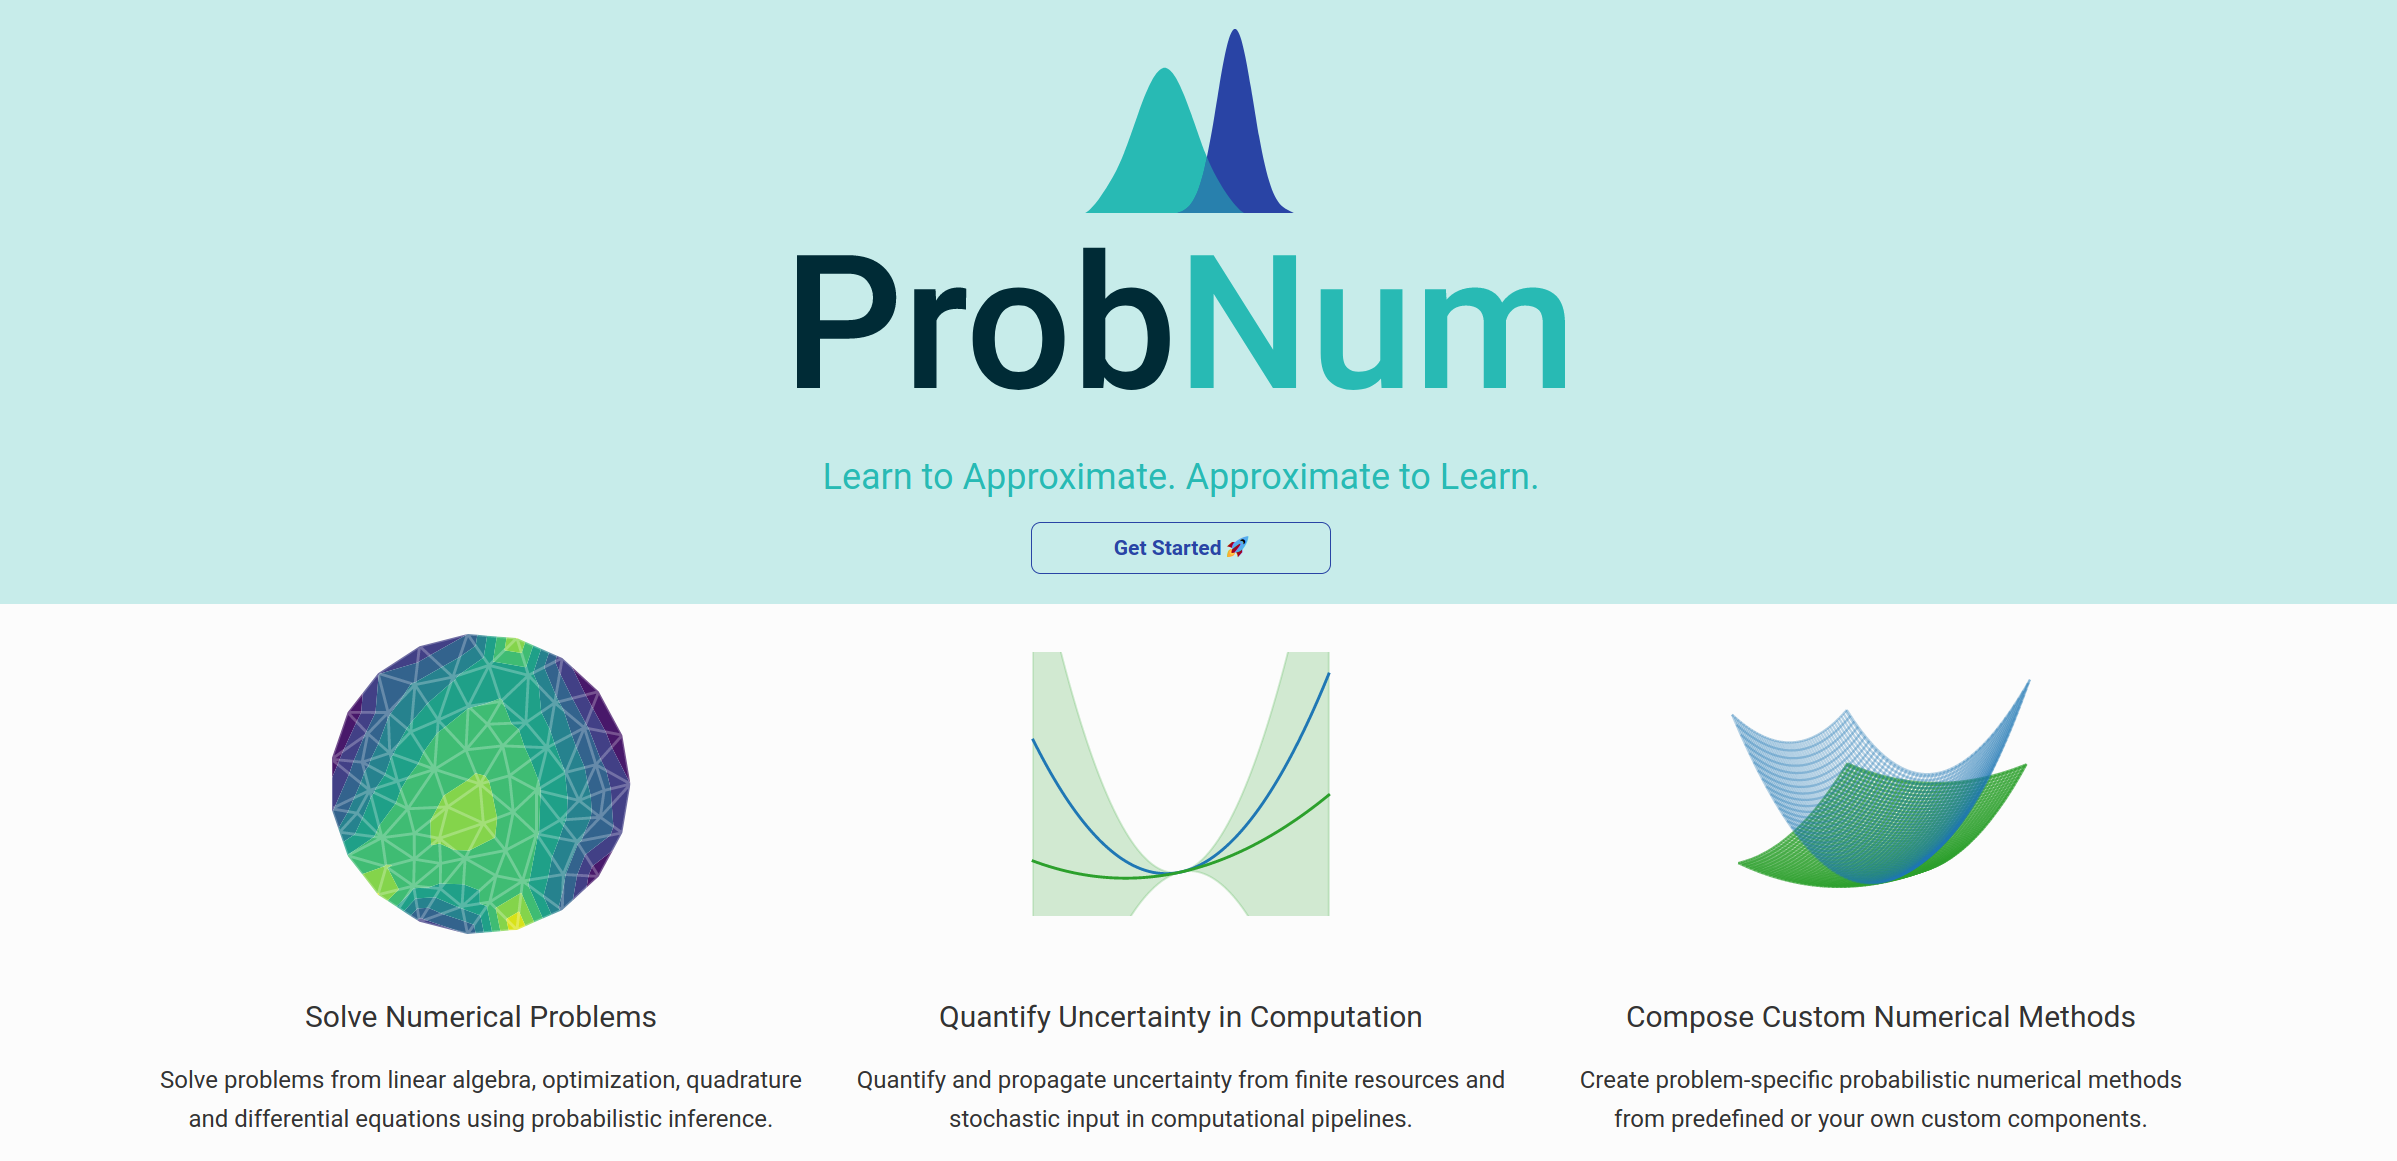
\includegraphics[width=1\paperwidth]{figures/probnum-docs.png}}
\end{frame}

\begin{frame}\frametitle{ProbNum}
	\framesubtitle{}

	\begin{columns}[totalwidth=\textwidth]
		\column{.6\textwidth}

		\emph{Problem}
		\begin{itemize}
			\item few implementations of probabilistic numerical methods
			\item not enough convincing applications available
		\end{itemize}

		\emph{Idea}
		\begin{itemize}
			\item lab / community-wide software framework for PN
		\end{itemize}

		\emph{Goals}
		\begin{itemize}
			\item \textit{promote PN research} via a useful code base
			\item \textit{simplify} the \textit{implementation} of new PN methods
			\item \textit{demonstrate} the \textit{use cases} of PN
			\item provide \textit{teaching} tools
		\end{itemize}

		\column{.3\textwidth}
		\centering
		\vspace{-3ex}
		\href{https://github.com/probabilistic-numerics/probnum/}{
\includegraphics[scale=0.3]{figures/probnum_logo_text.png}}
		
\includegraphics[width=\textwidth]{figures/probnum_contributors.png}
		%\vspace{-4ex}
		\begin{center}
			\begin{tikzpicture}[yscale=.6]
				%	    \filldraw[black] (2,0) rectangle (4,2);
				%	    \filldraw[gray] (0,2) rectangle (2,4);
				%	    \filldraw[gray] (2,2) rectangle (4,4);

				\draw[step=2cm,thick] (0,0) grid (4,4);

				\node[align=center] at (1,3) {Linear\\ Algebra};
				\node[align=center] at (3,3) {Quadrature};

				\node[align=center] at (3,1) {\textcolor{gray}{Bayesian}\\ \textcolor{gray}{Optimization}};
				\node[align=center] at (1,1) {Differential\\ Equations};
			\end{tikzpicture}
		\end{center}
	\end{columns}
	\vspace{1em}
	\ribbon{ProbNum on GitHub: {\small \url{https://github.com/probabilistic-numerics/probnum/}}}

\end{frame}

\subsection{Design Principles}

\begin{frame}[fragile]\frametitle{Design Principles of ProbNum}
	\framesubtitle{}

	\begin{columns}[totalwidth=\textwidth]
		\column{.7\textwidth}

		\emph{In- and Outputs:} PN Methods take random variables / processes as inputs and return random
		variables / processes as outputs.
		\vspace{2ex}

		\emph{Interface Design:} Drop-in replacement for NumPy / SciPy

		\begin{python}
			# Solve using NumPy
			x = np.linalg.solve(A, b)

			# Solve using ProbNum
			x_rv, _, _, info = pn.linalg.problinsolve(A, b)\end{python}
		\vspace{2ex}

		\emph{Implementation:} Compositionality enables custom PN Methods

		\begin{python}
			pn.linalg.ProbabilisticLinearSolver(
			problem=(A, b),
			state=(A_prior, Ainv_prior),
			policy=krylov,
			stopping_criterion=trace_Ainv_cov
			)\end{python}

		\column{.25\textwidth}
		\centering
		\vspace{-3ex}
		\href{https://github.com/probabilistic-numerics/probnum/}{
\includegraphics[scale=0.3]{figures/probnum_logo_text.png}}

	\end{columns}

\end{frame}

\section{Case Study}

\begin{frame}\frametitle{Case Study: ODE Filters}
	\framesubtitle{Solving ODEs with Uncertainty Estimation}

	\begin{center}
		\url{http://www.probabilistic-numerics.org/en/latest/tutorials.html}
	\end{center}

	\begin{center}
		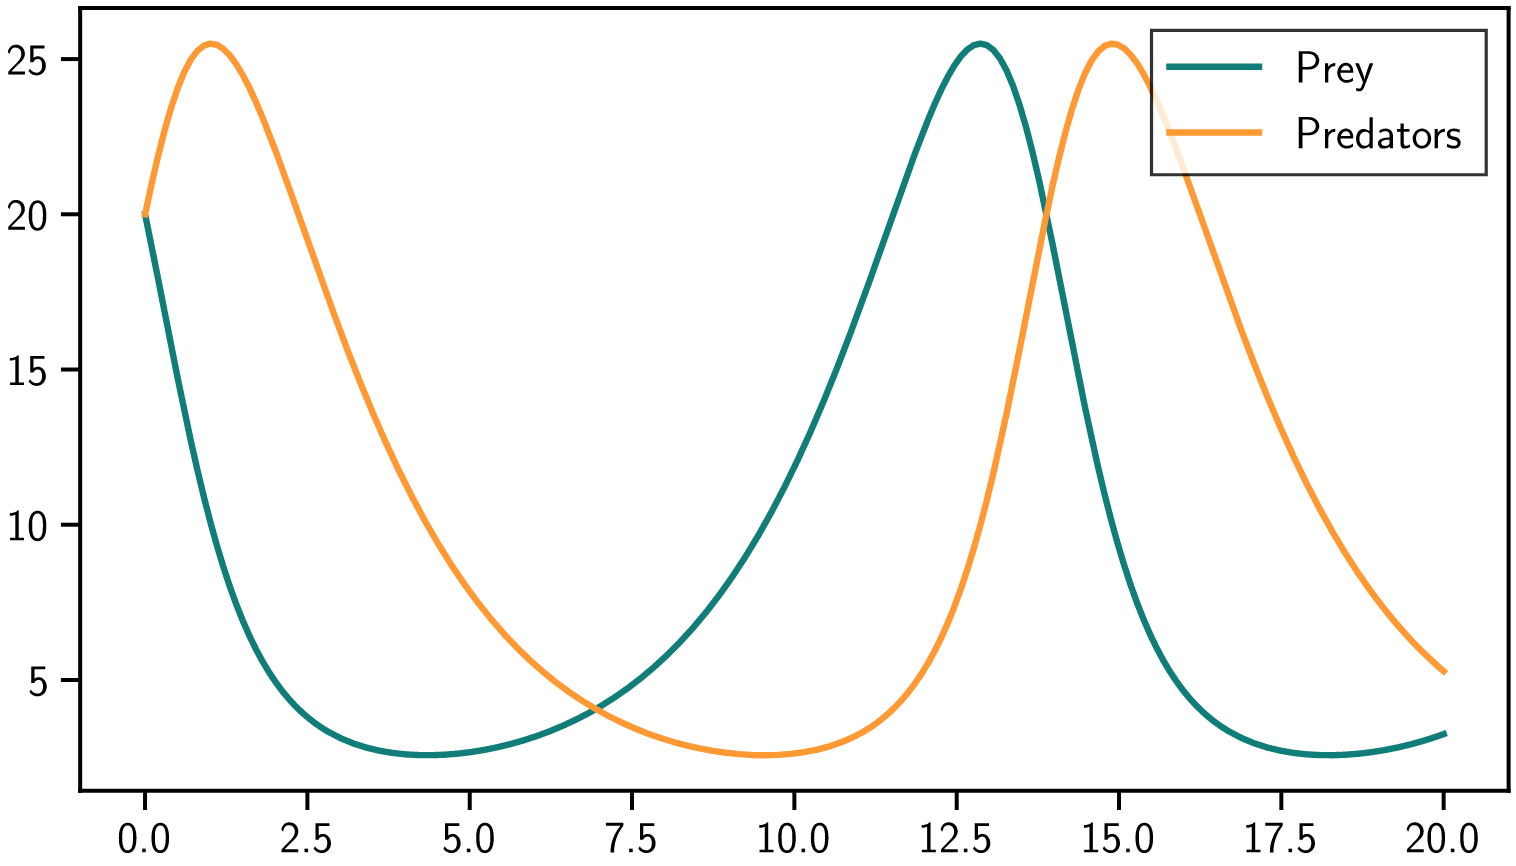
\includegraphics[width=0.75\textwidth]{figures/predator-prey.png}
	\end{center}

\end{frame}

\section{Conclusion}

\blackslidetext{
	\frametitle{Summary}

	\textbf{PN Methods - An Algorithmic View}
	\begin{itemize}
		\item implementing PN methods forces being precise about concepts
		\item abstract implementation surprisingly hard to define
		\item components of a PN method
		      \begin{itemize}
			      \item prior
			      \item policy
			      \item action and observation
			      \item posterior inference
			      \item stopping criterion
			      \item hyperparameter optimization
		      \end{itemize}
	\end{itemize}

	\whiteribbon{\centering Questions or Feedback?}

}

% References
\newcounter{references}
\setcounter{references}{\value{framenumber}} % Adjust frame counter to not include references

\begin{frame}[allowframebreaks]{References}
	\bibliographystyle{apalike}
	\bibliography{references}
\end{frame}

\setcounter{framenumber}{\value{references}}

\end{document}